% Auto-generated by the analysis pipeline — do not edit
% y > 0: Underreacts  |  y < 0: Overreacts
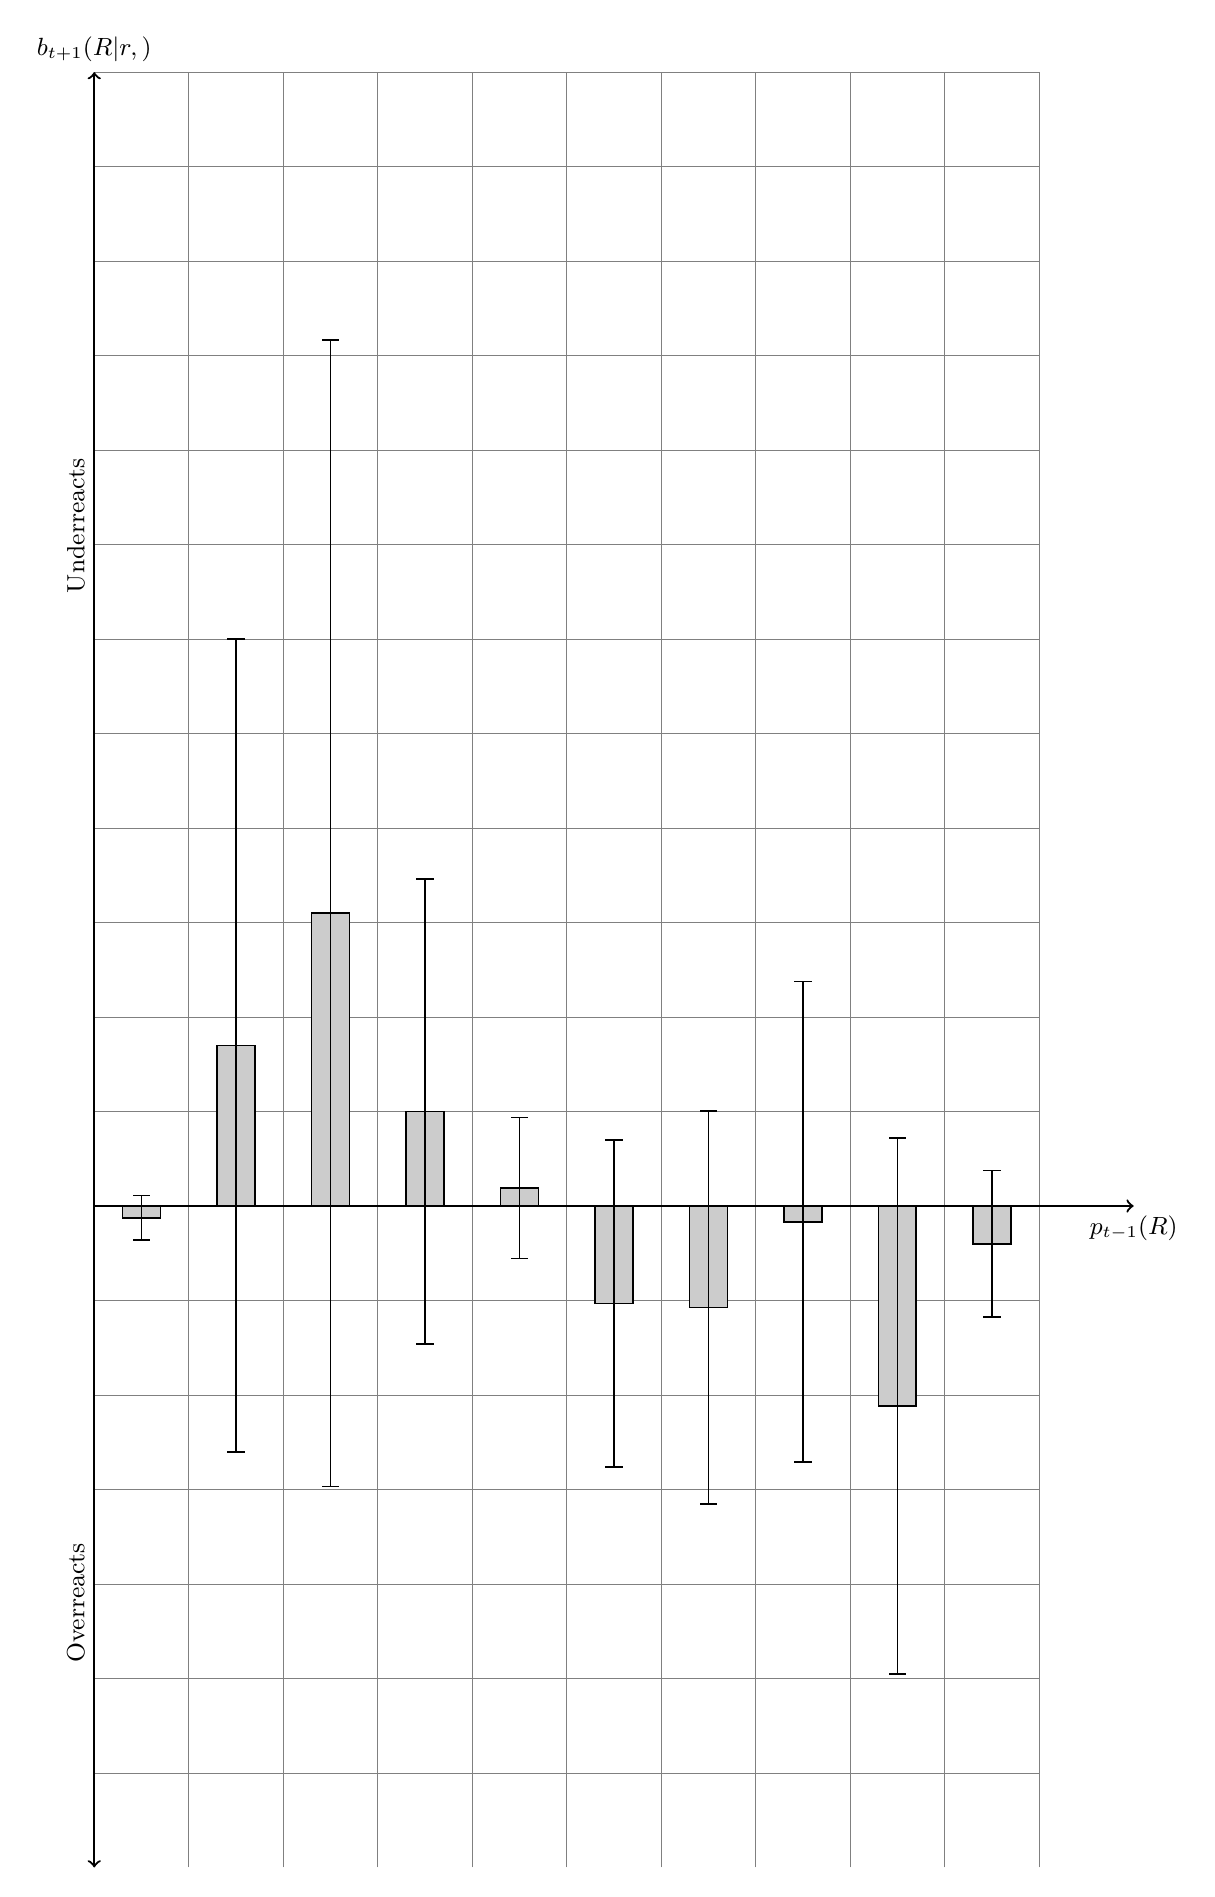
\begin{tikzpicture}[scale=12]
\draw[help lines,step=0.1] (0,-0.7) grid (1,1.2);
\filldraw[opaque,white!80!black] (0.03,0) rectangle (0.07,-0.0125);
\draw[line width=0.6] (0.03,0) rectangle (0.07,-0.0125);
\draw[line width=0.6,|-|] (0.05,-0.0370) -- (0.05,0.0120);
\filldraw[opaque,white!80!black] (0.13,0) rectangle (0.17,0.1700);
\draw[line width=0.6] (0.13,0) rectangle (0.17,0.1700);
\draw[line width=0.6,|-|] (0.15,-0.2612) -- (0.15,0.6012);
\filldraw[opaque,white!80!black] (0.23,0) rectangle (0.27,0.3100);
\draw[line width=0.6] (0.23,0) rectangle (0.27,0.3100);
\draw[line width=0.6,|-|] (0.25,-0.2976) -- (0.25,0.9176);
\filldraw[opaque,white!80!black] (0.33,0) rectangle (0.37,0.1000);
\draw[line width=0.6] (0.33,0) rectangle (0.37,0.1000);
\draw[line width=0.6,|-|] (0.35,-0.1466) -- (0.35,0.3466);
\filldraw[opaque,white!80!black] (0.43,0) rectangle (0.47,0.0190);
\draw[line width=0.6] (0.43,0) rectangle (0.47,0.0190);
\draw[line width=0.6,|-|] (0.45,-0.0566) -- (0.45,0.0946);
\filldraw[opaque,white!80!black] (0.53,0) rectangle (0.57,-0.1033);
\draw[line width=0.6] (0.53,0) rectangle (0.57,-0.1033);
\draw[line width=0.6,|-|] (0.55,-0.2773) -- (0.55,0.0706);
\filldraw[opaque,white!80!black] (0.63,0) rectangle (0.67,-0.1075);
\draw[line width=0.6] (0.63,0) rectangle (0.67,-0.1075);
\draw[line width=0.6,|-|] (0.65,-0.3164) -- (0.65,0.1014);
\filldraw[opaque,white!80!black] (0.73,0) rectangle (0.77,-0.0167);
\draw[line width=0.6] (0.73,0) rectangle (0.77,-0.0167);
\draw[line width=0.6,|-|] (0.75,-0.2718) -- (0.75,0.2385);
\filldraw[opaque,white!80!black] (0.83,0) rectangle (0.87,-0.2117);
\draw[line width=0.6] (0.83,0) rectangle (0.87,-0.2117);
\draw[line width=0.6,|-|] (0.85,-0.4961) -- (0.85,0.0727);
\filldraw[opaque,white!80!black] (0.93,0) rectangle (0.97,-0.0400);
\draw[line width=0.6] (0.93,0) rectangle (0.97,-0.0400);
\draw[line width=0.6,|-|] (0.95,-0.1184) -- (0.95,0.0384);
\draw[line width=0.8,->]  (0,0) -- (1.1,0) node[below] {\small{$p_{t-1}(R)$}};
\draw[line width=0.8,<->] (0,-0.7) -- (0,1.2) node[above] {\small{$b_{t+1}(R|r,\xmark)$}};
\draw (0,0.72) node[above,rotate=90] {\small{Underreacts}};
\draw (0,-0.42) node[above,rotate=90] {\small{Overreacts}};
% ADD THEORY CURVE BELOW
\end{tikzpicture}
